\paragraph{}
In today world we are surrounded by numbers of electronic devices that produce a lot of data every minute. A big part of these data ends up in huge data centres and waiting to be processed. However, it is impossible so that all of them are analysed by humans. It is also extremely hard to manually define and implement rules that can extract relevant information for further processing. Fortunately, these problems can be solved by involving machine learning (ML) techniques into data analysis. 

\paragraph{}
As Murphy states in his book \cite{ml_probabilistic},  ML can be defined as a set of methods and algorithms, that allows computers to automatically discover patterns in both structured and unstructured data and use these patterns to automatically derive rules for making further decisions. In subsequent sections, some of machine learning types, tasks and techniques are going to be discussed. 

\section{Types of machine learning}
\paragraph{}
In general, ML can be divided into three types - supervised, unsupervised and reinforcement learning. Difference between the types is mainly in data that are used for learning and each type is suitable for a different set of tasks. Although this work states only three types, a more detailed division can be found in the following book \cite{ml_foundations}.

\subsection{Supervised learning}
\paragraph{}
Supervised learning is a kind of ML where each example from training dataset consists of data itself (input) and a label (desired output). This type of learning suits very well for tasks such as classification or regression \cite{python_ml_2nd}.

\subsection{Unsupervised learning}
\paragraph{}
The second type of ML is called unsupervised learning and is characterized by a dataset which lacks information about desired output (label). The target of this kind of learning is to find important patterns that emerge in the given data. Unfortunately, an absence of knowledge of the true output represents a problem with evaluating learning performance \cite{ml_probabilistic}. This kind of ML is often used for clustering, dimensionality reduction and word embedding in the natural language processing field (chapter \ref{word_embedding}).

\subsection{Reinforcement learning}
\paragraph{}
In the case of reinforcement learning, the used dataset does not contain label in much the same way as in the case of unsupervised learning. The difference is, that the learner (so-called agent) can interact with its environment and receive feedback for his actions. This feedback consists of two parts. First is information telling the agent how did a state of the environment change. The second one is information about how successful his move was. This kind of information is called a reward \cite{ml_foundations} and the agent improves its behaviour to maximize it \cite{python_ml_2nd}. Scheme of interaction between the agent and the environment is depicted on the figure \ref{reinforcement_scheme}. Reinforcement learning can be
used for example for robot motion control or playing games.

\begin{figure}[!h]
	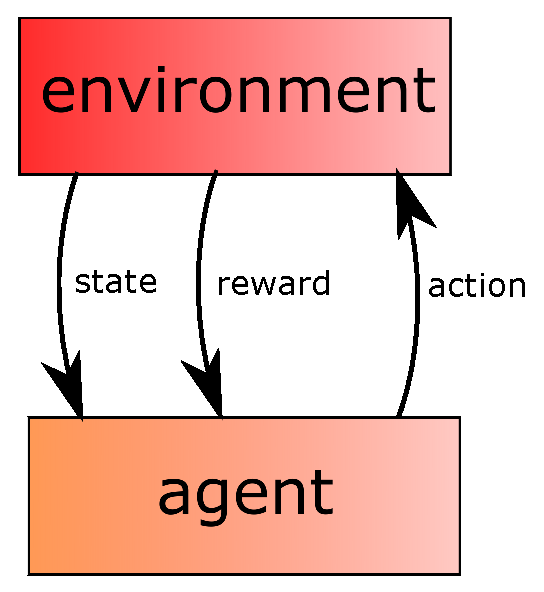
\includegraphics[width=5cm]{reinforcement.eps}
	\centering
	\caption{Scheme of reinforcement learning}
	\label{reinforcement_scheme}
\end{figure}

\section{Machine learning tasks}\label{ML_tasks_section}
\paragraph{}
Generally speaking, ML aims to create systems that can make as accurate predictions as possible for unseen data. Concrete tasks can be divided into few classes - classification, regression and clustering \cite{ml_foundations}. These three classes are going to be further described in subsequent subsections.

\subsection{Classification}
\paragraph{}
 target of classification is to find a function $f$ whose input is a data item to be classified and an output is a number $c \in [0,C-1] \cap \mathbb{Z}$, where $C$ is a number of classes into which data shall be classified. In other words, we try to find a mapping between each input and its correct class. \cite{ml_probabilistic}

\paragraph{}
While talking about classification, we distinguish three types. The first one is a binary classification which is characterized by a number of possible classes equal to two. It means that the input can be assigned to two different classes only (for example true or false). Otherwise, when C is greater than two, we are talking about multi-class classification. Last but not least, we also identify multi-label classification which is a case where multiple classes can be assigned to one input. \cite{ml_probabilistic}

\paragraph{}
A good example of multi-class classification is a classification of handwritten digits from MNIST dataset \cite{mnist_page}. In this problem, we are given a greyscale picture 28x28 pixels (such as on figure \ref{mnist_example}) and the task is to predict a correct digit (0-9). 

\begin{figure}[!h]
	\includegraphics[width=10cm]{mnist.eps}
	\centering
	\caption{Example of digits from MNIST dataset}
	\label{mnist_example}
\end{figure}

\subsection{Regression}
\paragraph{}
In case of classification, a target was to find the function $f$ whose output was a discrete class whereas in regression analysis we aim to obtain a function $f$ with continuous output. In the other words, we try to capture the continuous dependence of output on input. Thanks to such function we can approximate or predict output for inputs that were never seen by our ML model. \cite{python_ml_2nd}

\paragraph{}
To describe  regression more in detail let's imagine that we have a set of points $[x_i, y_i], i=0 ... n$,  and we want to find an equation of a curve that approximates the given set of points in some optimal way. For example, in the case of L2 approximation, the measure of optimality ($L$) is the sum of squares of deviations of all the given points from the curve in the y-axis (equation \ref{L2_approximation}). The solution of regression analysis is to find parameters of the curve that minimize the $L$.

\begin{equation}
	L = \sum_{i=0}^{n} (y_i - f(x_i))^2
	\label{L2_approximation}
\end{equation} 

\subsection{Clustering}
\paragraph{}
As explained in the book by Sebastian Raschka and Vahid Mirjalili \cite{python_ml_2nd}, clustering is an unsupervised technique for partitioning data items into groups that share some signs of similarity and appears to be quite different to the items in other groups. This technique can be extremely helpful for instance with identifying communities among users of social networks. Example of clustering can be found on figure \ref{clustering_visualization}.

\begin{figure}[!h]
	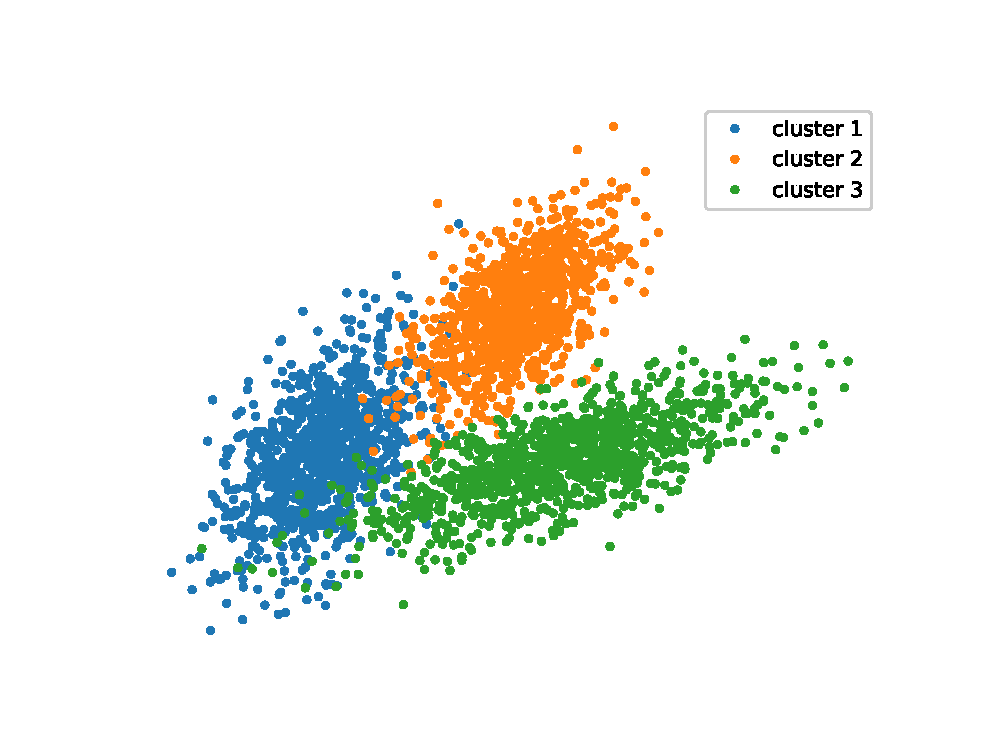
\includegraphics[width=10cm]{clustering.eps}
	\centering
	\caption{Visualization of data partitioning into 3 clusters}
	\label{clustering_visualization}
\end{figure}

\section{Examples of classification techniques}
\paragraph{}
Since the majority of this work will deal with classification problem a short overview of chosen classification methods/algorithms is given in following subsections.

\subsection{Decision Trees}
\paragraph{}
A decision tree (or classification tree) is a ML technique which uses a set of decisions organized into a tree structure to predict the class for the given input. Each node inside the classification tree represents a decision/condition (e.g. 'age >= 30'), whereas leafs represent resulted class. An organization and thresholds of all the decisions are induced from a training dataset using known algorithms such as C4.5. \cite{decision_trees}

\paragraph{}
The classification procedure always starts from the root node. At each node, the condition is evaluated and the computation continues to the underlying node which corresponds to the result of the previous decision. When one of the leaves if reached, the computation ends and the class represented by the leaf is stated as a result of classification. An example of classification using decision tree can be found on figure \ref{decision_tree_example}.

\begin{figure}[!h]
	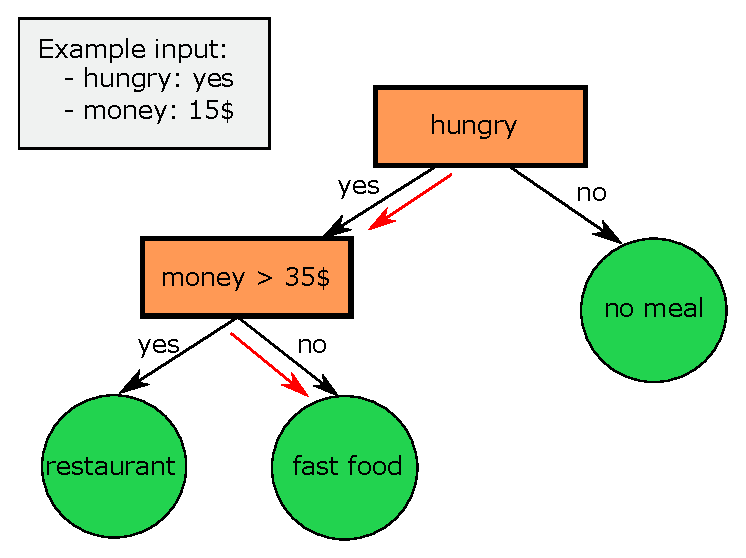
\includegraphics[width=8cm]{decision_tree.eps}
	\centering
	\caption{Example of classification tree of where to eat based on budged and current hunger}
	\label{decision_tree_example}
\end{figure}

\subsection{K - Nearest Neighbours}
\paragraph{}
K - Nearest Neighbours (KNN) is a very simple classification algorithm which searches for $K$ data items from a training dataset that are the nearest to the classified example. Resulted class is then chosen as the most frequent one among the $K$ selected items. Unfortunately, as explained in \cite{ml_probabilistic}, KNN becomes inapplicable for very large datasets or  high dimensional inputs.

\subsection{Support Vector Machine}
\paragraph{}
Support Vector Machine (SVM) is a ML algorithm for finding an optimal separating hyperplane for a given set of training examples. The separating hyperplane is considered as optimal if it maximizes a margin between points that are closest to the hyperplane and the hyperplane itself \cite{ml_foundations}. These closest points are called support vectors. The figure \ref{svm_example} shows an optimal hyperplane for a linearly separable set of points with support vectors lying on the dashed lines. 

\begin{figure}[!h]
	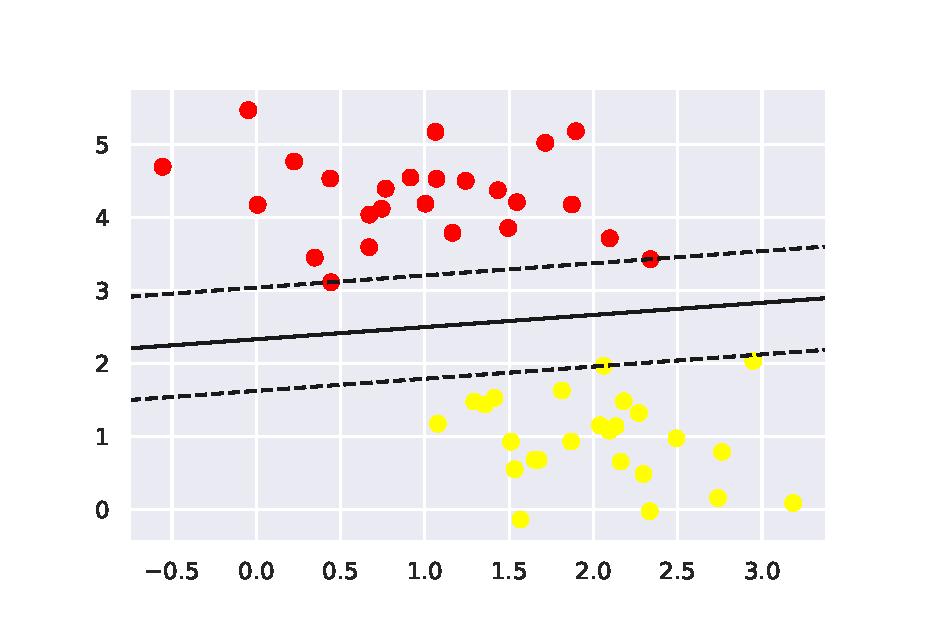
\includegraphics[width=9cm]{svm.eps}
	\centering
	\caption{Example of optimal separating hyperplane in linearly separable set of points}
	\label{svm_example}
\end{figure}

While talking about SVMs, two different cases can be distinguished. The simpler case is when the training set is linearly separable. In this case, the parameters of optimal hyperplane are found using an optimization method. However, in the case where a linear separator does not exist, a kernel function which transforms the set of points into linearly separable space must be applied to all  of the points before attempting to find the hyperplane \cite{ml_foundations}. Figures \ref{smv_non_sep} and \ref{svm_kernel} show the non-linearly separable set of points before and after applying the kernel function. 

\begin{figure}[!h]
	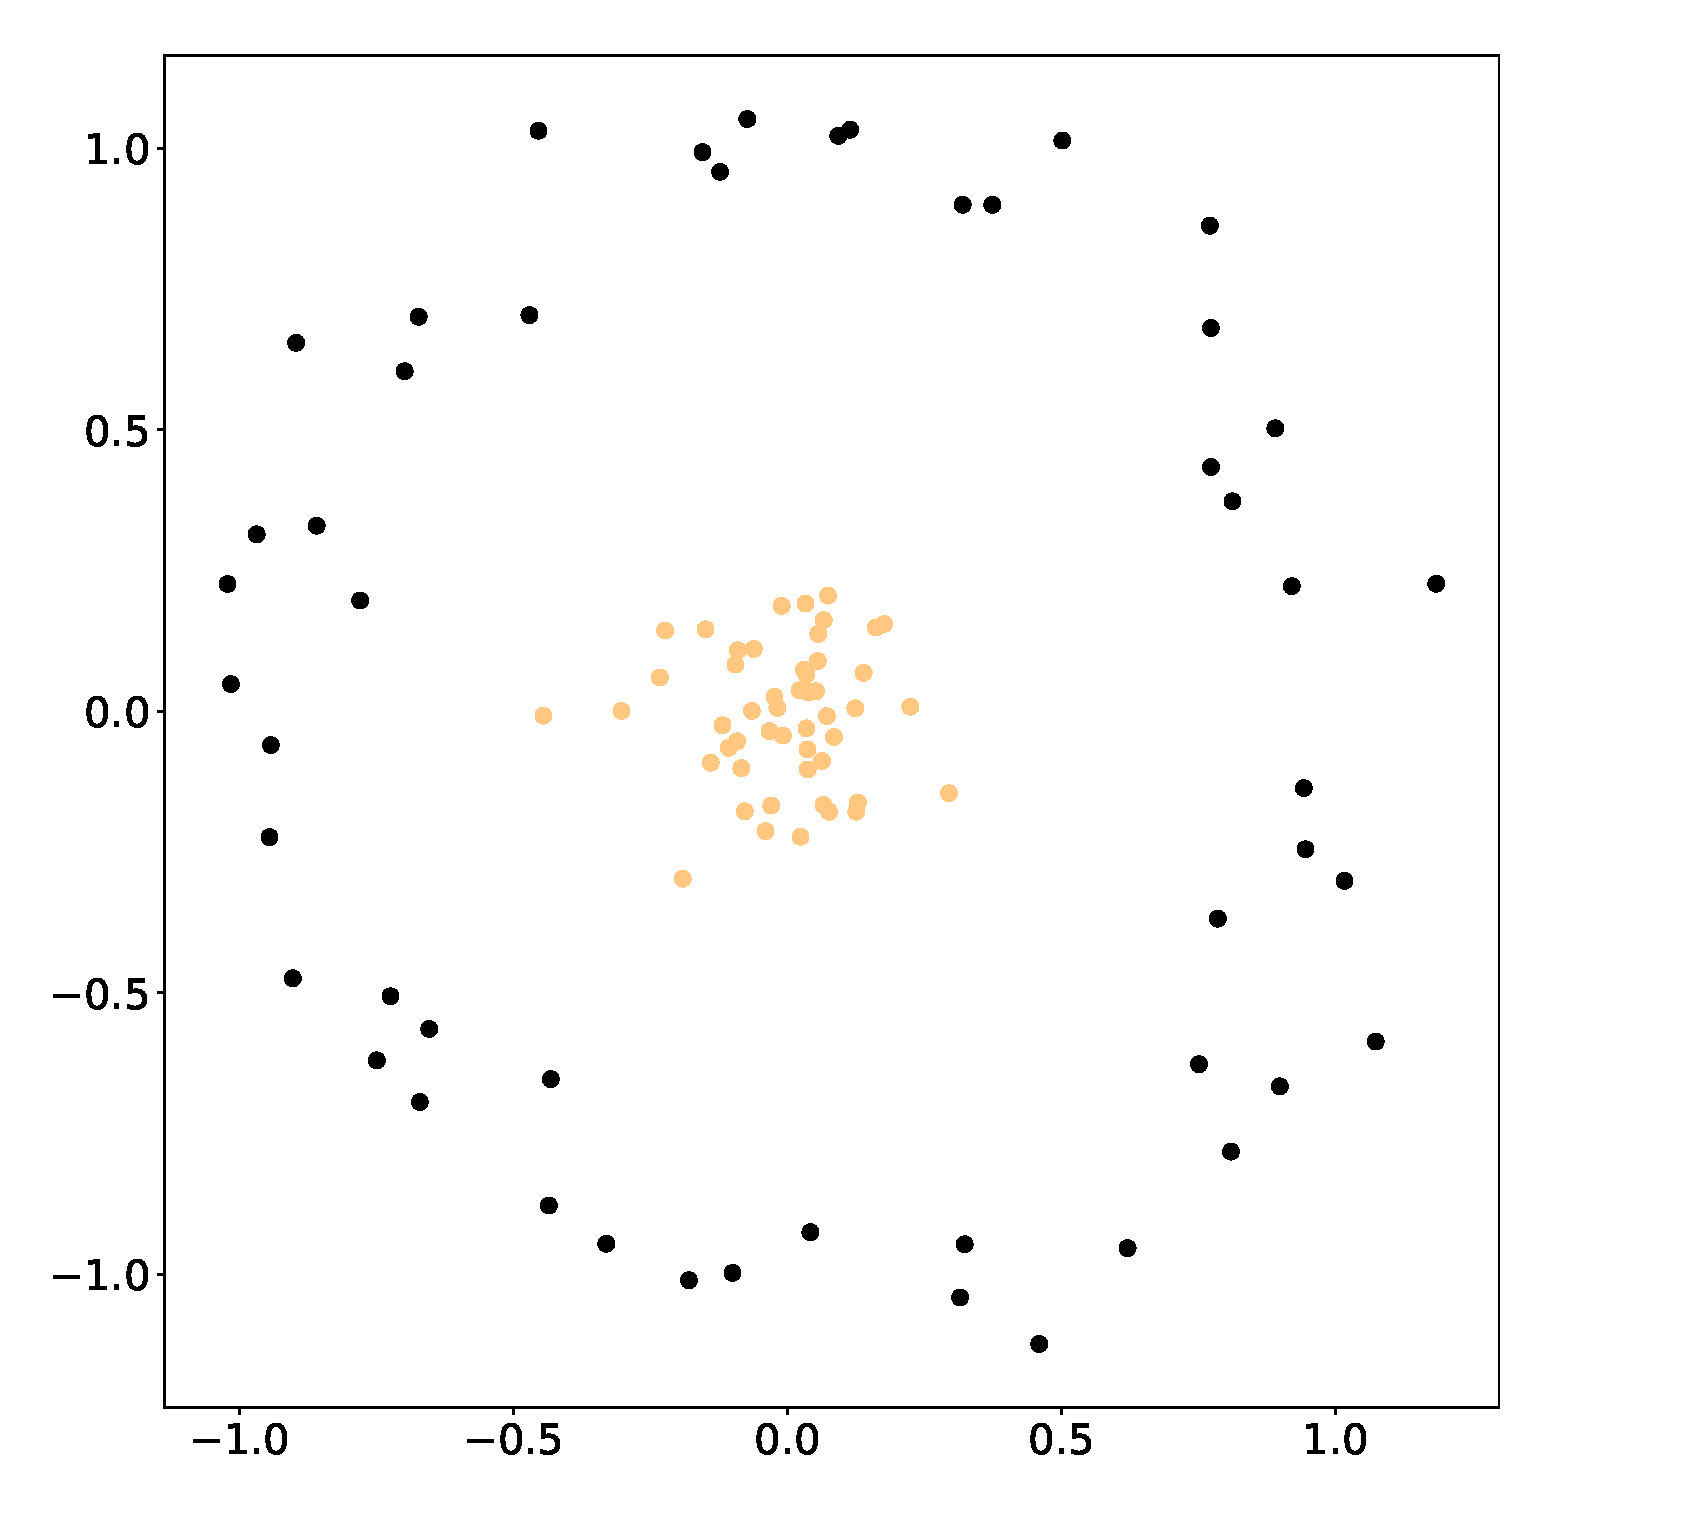
\includegraphics[width=8cm]{svm_non_sep.eps}
	\centering
	\caption{Linearly non separable set of points}
	\label{smv_non_sep}
\end{figure}

\begin{figure}[!h]
	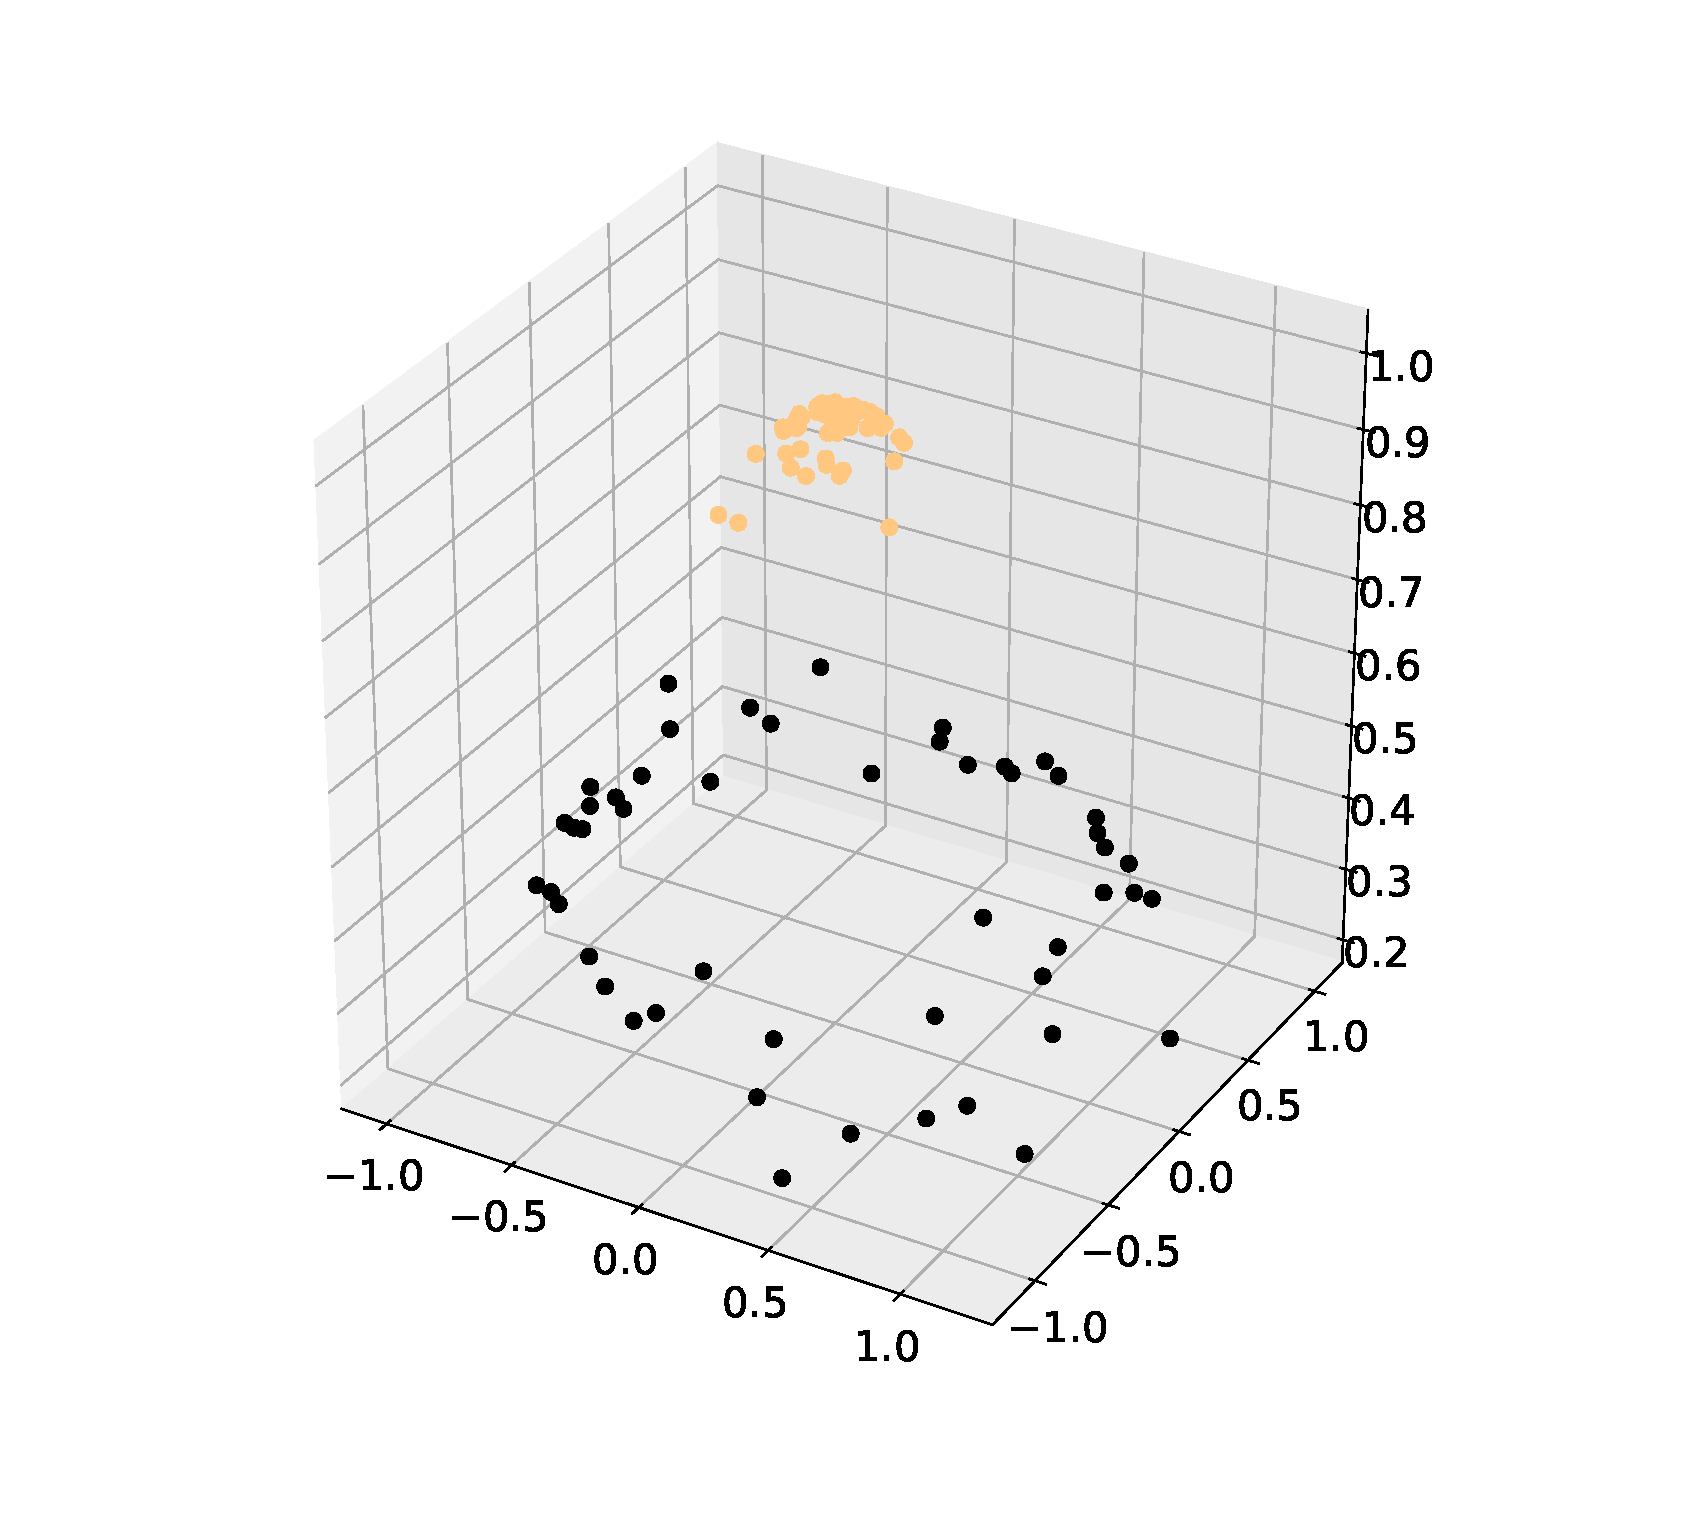
\includegraphics[width=10cm]{svm_kernel.eps}
	\centering
	\caption{Linearly separable set of points after applying kernel function}
	\label{svm_kernel}
\end{figure}

\subsection{Deep learning}
\paragraph{}
Deep learning is a subset of machine learning techniques based on artificial neural networks which are described in detail in chapter \ref{NN}.